\def\r{2}
\def\rr{1.5}
\tdplotsetmaincoords{60}{125}

\pgfdeclareradialshading[tikz@ball]{ball}{\pgfqpoint{-20bp}{20bp}}{%
    color(0bp)=(tikz@ball!0!white);
    color(17bp)=(tikz@ball!0!white);
    color(21bp)=(tikz@ball!70!black);
    color(25bp)=(black!70);
    color(30bp)=(black!70)}


\definecolor{mediumtaupe}{rgb}{0.4, 0.3, 0.28}
\def\colorlist{{"red", "blue", "green!80!black", "brown!50!orange"}}

\vspace{-1em}
\hspace{-3em}
\begin{tikzpicture}[tdplot_main_coords]
    
%    \foreach \i in {-75, -45, ..., 75}{
        %\tdplotCsDrawLatCircle[thin, black!20]{\r}{\i}
%    }

 %   \foreach \i in {0, 60, ..., 150}{
        %\tdplotCsDrawLonCircle[thin, black!10]{\r}{\i}
 %   }
%    \tdplotCsDrawPoint[black!50]{0}{0}{0}


    \node[inner sep=0pt] (ballpic) at (0.555,0.55)
    {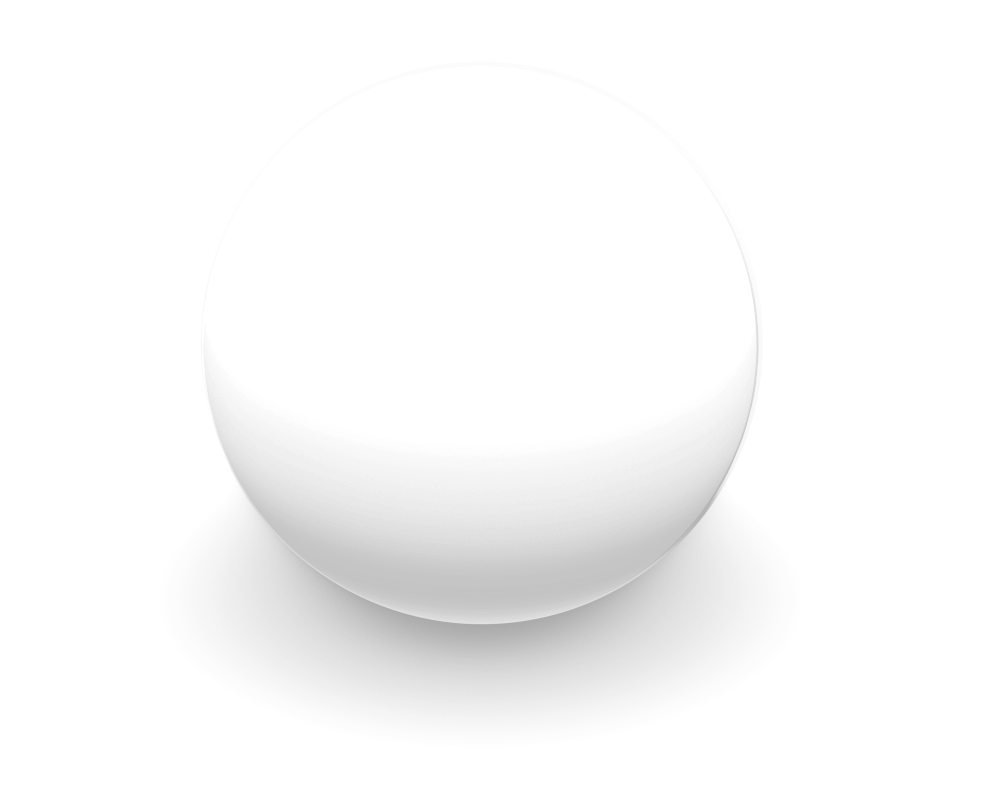
\includegraphics[width=205pt]{pics/ballrender.png}};

    \fill[black!50] (0, 0) circle (0.05);
        
    \tdplotCsDrawCircle[mediumtaupe, thin, gray,
    tdplotCsFill/.style = {opacity = 0},
    tdplotCsBack/.style = {white}]{\r}{0}{0}{45}
    \foreach \i in {0, 1, ..., 3}{        

        \pgfmathparse{\colorlist[\i]}
        \edef\col{\pgfmathresult}
        
        \tdplotCsDrawPoint[\col]{\r}{54 * \i - 40}{45.5}
        
        \tdplotCsDrawCircle[
            \col,
            thick,
            tdplotCsBack/.style = {thin, densely dotted},
            tdplotCsFill/.style = {opacity = 0.08}]{\r}{54 * \i - 40}{-50}{0}
    }
    \draw[gray, tdplot_screen_coords] (0, 0, 0) circle (\r);

    \begin{scope}[tdplot_screen_coords, shift = {(2.9, 1)}]
        \pic {universe-rect = {2}};
        \foreach \i in {0, 1, 2, 3}{
            \foreach \j in {0, 1, 2, 3}{
                \ifthenelse{\i = \j}{
                    \pgfmathparse{\colorlist[\j]}
                    \edef\col{\pgfmathresult}
                    \node at (0.25 + 0.5 * \i, -0.25 - 0.5 * \j) {\textcolor{\col!80!black}{1}};
                }{
                    \node at (0.25 + 0.5 * \i, -0.25 - 0.5 * \j) { }; % NH: Removed 0 entries for readability
                }
            }
        }
    \end{scope}
    \node[tdplot_screen_coords] at (2.5, 0) {$\cong$};
    

    \begin{scope}[tdplot_screen_coords, shift = {(0, -5)}]
        \draw[thick] (0, 0) circle (\rr);

       	\foreach \i in {0, 1, 2, 3}{
            \pgfmathparse{\colorlist[\i]}
            \edef\col{\pgfmathresult}

            \draw[\col, thick] (20 + 30 * \i:\rr + 0.25) -- (20 + 30 * \i + 180:\rr + 0.5);
            \fill[\col] (35 + 30 * \i:\rr) circle (2pt);
        }

        \begin{scope}[tdplot_screen_coords, shift = {(2.4, 1)}]
            \pic {universe-rect = {2}};
            \foreach \i in {0, 1, 2, 3}{
                \foreach \j in {0, 1, 2, 3}{
                    \ifthenelse{\i > \j}{
                        \node at (0.25 + 0.5 * \i, -0.25 - 0.5 * \j) { }; % NH: Removed 0 entries for readability
                    }{
                        \pgfmathparse{\colorlist[\i]}
                        \edef\col{\pgfmathresult}
                        \node at (0.25 + 0.5 * \i, -0.25 - 0.5 * \j) {\textcolor{\col!80!black}{1}};
                    }
                }
            }
        \end{scope}
        \node[tdplot_screen_coords] at (2, 0) {$\cong$};
    \end{scope}
\end{tikzpicture}
\vspace{-3.5em}